\documentclass{scrartcl}
\usepackage[a4paper, total={6in, 10in}]{geometry}
\usepackage[ngerman]{babel}

\usepackage{tabularx} % Für bessere Tabellen
\usepackage{booktabs} % Für professionelle Tabellenlinien
\usepackage{xcolor}
\usepackage{graphicx}

\usepackage{amsmath}
\usepackage{amssymb}
\usepackage{algorithm}
\usepackage{algpseudocode}

\makeatletter
\renewcommand{\ALG@name}{Algorithmus}
\makeatother
\algrenewcommand\algorithmicrequire{\textbf{Eingabe:}}
\algrenewcommand\algorithmicensure{\textbf{Ausgabe:}}

\title{Matrixmultiplikation von \normalfont\scshape{Strassen}}
\author{Stephan Epp}
\date{\today}

\begin{document}
\maketitle
Beim Algorithmus von \textsc{Strassen} für die Multiplikation von zwei $n \times n$ Matrizen lautet die Rekurrenz zur Ermittlung der Laufzeit $T(n)$ des Algorithmus
\begin{align*}
	T(n) = 7 \: T(\tfrac{n}{2}) + c\: n^2.
\end{align*}
Der Algorithmus halbiert in jedem rekursiven Aufruf die beiden $n \times n$ Matrizen zu vier $\tfrac{n}{2} \times \tfrac{n}{2}$ Matrizen. Substituieren wir $n$ durch $\tfrac{n}{2}$, erhalten wir für
\begin{align*}
	T(\tfrac{n}{2}) &= 7 \: T(\tfrac{n}{4}) + c(\tfrac{n}{2})^2 = 7 \: T(\tfrac{n}{4}) + \tfrac{c}{4}n^2.
\end{align*}
Nach dem \textit{ersten} rekursiven Aufruf erhalten wir mit $T(\frac{n}{2})$ eingesetzt in $T(n)$ dann
\begin{align*}
	T(n) &= 7 \: (7 \: T(\tfrac{n}{4}) + \tfrac{c}{4} \: n^2) + c n^2 \\
	&= 7^2\: T(\tfrac{n}{4}) + \tfrac{7}{4} \: cn^2 + c n^2.
\end{align*}
Mit dem \textit{zweiten} rekursiven Aufruf werden die vier $\tfrac{n}{2} \times \tfrac{n}{2}$ Matrizen wieder halbiert zu acht $\tfrac{n}{4} \times \tfrac{n}{4}$ Matrizen. Damit ist
\begin{align*}
	T(\tfrac{n}{4}) &= 7 \: T(\tfrac{n}{8}) + c(\tfrac{n}{4})^2 = 7 \: T(\tfrac{n}{8}) + \tfrac{c}{16}n^2.
\end{align*}
Wird $T(\tfrac{n}{4})$ eingesetzt in $T(n)$ ergibt sich
\begin{align*}
	T(n) &= 7^2\: (7 \: T(\tfrac{n}{8}) + \tfrac{c}{16}n^2) + \tfrac{7}{4}cn^2 + c n^2 \\
	&= 7^3\: T(\tfrac{n}{2^3}) + \tfrac{7^2}{4^2}cn^2 + \tfrac{7}{4}cn^2 + c n^2.
\end{align*}
Betrachten wir nun den $k$-ten rekursiven Aufruf finden wir für 
\begin{align*}
	T(n) = 7^k \: T \: \big(\tfrac{n}{2^k}\big) + cn^2 \: \sum_{i = 0}^{k-1} \bigg(\frac{7}{4}\bigg)^i.
\end{align*}
Zur Vereinfachung belassen wir es bei dem $k$-ten rekursiven Aufruf auch in $T(n)$ bei $k$ und nicht $k + 1$. Kleinere Matrizen als $1 \times 1$ Matrizen gibt es nicht, daher können die $n \times n$ Matrizen nur $k$ mal halbiert werden. Der größte Wert, den $k$ annehmen kann, ist $k = \log_{2}n$. Damit ist
\begin{align*}
	\vphantom{\rule{0pt}{2.5ex}} T(n) &= 7^{\log_{2}n} \: T\Big(\frac{n}{2^{\log_{2}n}}\Big) + cn^2 \: \sum_{i = 0}^{\log_{2}n-1} \left(\tfrac{7}{4}\right)^i \\
	\vphantom{\rule{0pt}{2.5ex}} &= n^{\log_{2}7} \: T(1) + cn^2 \:\frac{\left(\tfrac{7}{4}\right)^{\log_{2}n} - 1}{\tfrac{7}{4} - 1} \\
	\vphantom{\rule{0pt}{2.5ex}} &= O\left(n^{2.8074}\right) + cn^2 \left(\tfrac{7}{4}\right)^{\log_{2}n} \\
	\vphantom{\rule{0pt}{2.5ex}} &= O\left(n^{2.8074}\right) + cn^2 \cdot n^{\log_{2}\tfrac{7}{4}} \\
	\vphantom{\rule{0pt}{2.5ex}} &= O\left(n^{2.8074}\right) + cn^{2.8074} \\
	\vphantom{\rule{0pt}{2.5ex}} &= O\left(n^{2.8074}\right).
\end{align*}

\section{Algorithmus}
Es folgt der Algorithmus \ref{alg:strassen} von \textsc{Strassen}  als Pseudocode. Als Eingabe erhalten wir zwei $n \times n$ Matrizen. Der Einfachheit halber wird angenommen, dass $n$ eine Zweierpotenz ist. Zu Beginn prüfen wir, ob die Größe der Matrizen bereits den Wert $1$ hat. Haben die Matrizen den Wert $1$, geben wir das Produkt $A B$ zurück.
\begin{algorithm}
	\caption{\textsc{Strassen}$(A, B)$}
	\label{alg:strassen}
	\begin{algorithmic}[1]
		\Require $\langle A, B \rangle$, mit $n \times n$ Matrizen $A$, $B$, $n = 2^k$, $k \in \mathbb{N}$
		\Ensure $\langle C \rangle$, mit Produktmatrix $C = AB$
		\If{$n = 1$} $C = AB$ %\Comment{Skalarmultiplikation}
		\State \textbf{return} $C$
		\EndIf
		%\Comment{Matrizen in $n/2 \times n/2$ Blöcke unterteilen}
		\State $A = \begin{pmatrix} A_{11} & A_{12} \\ A_{21} & A_{22} \end{pmatrix}$
		\State $B = \begin{pmatrix} B_{11} & B_{12} \\ B_{21} & B_{22} \end{pmatrix}$
		%\Comment{Berechne die 7 Produkte rekursiv}
		\State $P_1 = \textsc{Strassen}(A_{11} + A_{22}, B_{11} + B_{22})$
		\State $P_2 = \textsc{Strassen}(A_{21} + A_{22}, B_{11})$
		\State $P_3 = \textsc{Strassen}(A_{11}, B_{12} - B_{22})$
		\State $P_4 = \textsc{Strassen}(A_{22}, B_{21} - B_{11})$
		\State $P_5 = \textsc{Strassen}(A_{11} + A_{12}, B_{22})$
		\State $P_6 = \textsc{Strassen}(A_{21} - A_{11}, B_{11} + B_{12})$
		\State $P_7 = \textsc{Strassen}(A_{12} - A_{22}, B_{21} + B_{22})$
		% \Comment{Berechne die Blöcke von $C$}
		\State $C_{11} = P_1 + P_4 - P_5 + P_7$
		\State $C_{12} = P_3 + P_5$
		\State $C_{21} = P_2 + P_4$
		\State $C_{22} = P_1 - P_2 + P_3 + P_6$
		\State \textbf{return} $C = \begin{pmatrix} C_{11} & C_{12} \\ C_{21} & C_{22} \end{pmatrix}$
	\end{algorithmic}
\end{algorithm}
In Zeile 4 und 5 werden die Matrizen $A$ und $B$ so definiert, dass in den Zeilen 6 bis 12 die sieben Matrixmultiplikationen jeweils durchgeführt werden. In den Zeilen 13 bis 16 werden 4 Matrizen $C_{ij}$ durch Addition und Subtraktion der Matrizen $A_{ij}$ berechnet und in Zeile 17 Matrix $C$ als Ergebnis zurückgegeben.

Als Idee zum Beweis der Korrektheit betrachten wir das Produkt $A \cdot B$ der zwei Matrizen $A$ und $B$ mit
\begin{align*}
	A = \begin{pmatrix} a & b \\ c & d \end{pmatrix} \quad \text{und} \quad B = \begin{pmatrix} e & f \\ g & h \end{pmatrix}.
\end{align*}
Zur Vereinfachung beinhalten die Matrizen nur skalare Werte. Das Ergebnis $C = A \cdot B$ ist
\begin{align*}
	C = \begin{pmatrix} ae + bg & af + bh \\ ce + dg & cf + dh \end{pmatrix}.
\end{align*}
Der Algorithmus von \textsc{Strassen} berechnet $P_i$ mit
\begin{align*}
	P_1 &= \textsc{Strassen}(a + d, e + h) && = ae + ah + de + dh\\
	P_2 &= \textsc{Strassen}(c + d, e) && = ce + de \\
	P_3 &= \textsc{Strassen}(a, f - h) && = af - ah\\
	P_4 &= \textsc{Strassen}(d, g - e) && = dg - de \\
	P_5 &= \textsc{Strassen}(a + b, h) && = ah + bh \\
	P_6 &= \textsc{Strassen}(c - a, e + f) && = ce + cf - ae - af\\
	P_7 &= \textsc{Strassen}(b - d, g + h) && = bg + bh - dg - dh.
\end{align*}
Dann werden $C_{ij}$ berechnet mit
\begin{align*}
	C_{11} & = P_1 + P_4 - P_5 + P_7 && = ae + bg\\
	C_{12} & = P_3 + P_5 && = af + bh\\
	C_{21} & = P_2 + P_4 && = ce + dg\\
	C_{22} & = P_1 - P_2 + P_3 + P_6 && = cf + dh,
\end{align*}
wobei z.B. $ C_{11} = (ae + ah + de + dh) + (dg - de) - (ah + bh) + (bg + bh - dg - dh) = ae + bg$. Für einen formalen Beweis der Korrektheit verzichten wir auf die vollständige Induktion über $n \in \mathbb{N}$ der $n \times n$ Matrizen.

\section{Experimentelle Ergebnisse in Python}
Um die theoretische Laufzeitanalyse von \textsc{Strassen}s Algorithmus zu überprüfen, wurde eine Python-Implementierung des Algorithmus erstellt und deren Performance mit der einer Standard-Matrixmultiplikation verglichen. Die Experimente wurden für Matrizen unterschiedlicher Größe ($n$) durchgeführt, wobei $n$ von 4 bis 256 in Schritten von 4 variiert wurde. Für jede Matrixgröße wurden 5 Messungen (Trials) durchgeführt und die durchschnittliche Laufzeit ermittelt.
\begin{table}[h!]
	\centering
	\caption{Vergleich der Laufzeiten von Standard- und \textsc{Strassen}-Matrixmultiplikation}
	\label{tab:strassen_results}
	\begin{tabularx}{\textwidth}{l | X | X}
		\toprule\midrule[\heavyrulewidth]
		$\mathbf{n}$ & \textbf{Standard Avg Time (s)} & \textbf{Strassen Avg Time (s)} \\
		\midrule
		4 & 0.000027 & 0.000045 \\
		8 & 0.000101 & 0.000142 \\
		12 & 0.000312 & 0.000698 \\
		16 & 0.000708 & 0.000808 \\
		20 & 0.001350 & 0.004538 \\
		24 & 0.002304 & 0.004827 \\
		28 & 0.003644 & 0.005236 \\
		\vdots & \vdots & \vdots \\
		% 32 & 0.005369 & 0.005674 \\
		% 36 & 0.007291 & 0.035827 \\
		% 40 & 0.010007 & 0.036722 \\
		% 44 & 0.013256 & 0.037815 \\
		% 48 & 0.017039 & 0.038888 \\
		52 & 0.021834 & 0.034057 \\
		\textcolor{red}{56} & \textcolor{red}{0.013749} & \textcolor{red}{0.020460} \\
		60 & 0.016938 & 0.020990 \\
		\vdots & \vdots & \vdots \\
		% 64 & 0.020041 & 0.021484 \\
		% 68 & 0.024157 & 0.133145 \\
		% 72 & 0.028486 & 0.133083 \\
		% 76 & 0.033549 & 0.143920 \\
		% 80 & 0.039826 & 0.141013 \\
		% 84 & 0.045262 & 0.141792 \\
		% 88 & 0.051738 & 0.152629 \\
		% 92 & 0.059471 & 0.146050 \\
		% 96 & 0.067689 & 0.147936 \\
		% 100 & 0.076471 & 0.162647 \\
		% 104 & 0.087148 & 0.154874 \\
		% 108 & 0.095150 & 0.155554 \\
		% 112 & 0.107501 & 0.158186 \\
		% 116 & 0.118892 & 0.171497 \\
		% 120 & 0.131730 & 0.165475 \\
		% 124 & 0.148736 & 0.166968 \\
		% 128 & 0.161912 & 0.179074 \\
		% 132 & 0.175445 & 0.999888 \\
		% 136 & 0.191708 & 1.045382 \\
		% 140 & 0.217163 & 1.082742 \\
		% 144 & 0.233093 & 1.084697 \\
		% 148 & 0.256793 & 1.078266 \\
		% 152 & 0.272154 & 1.076065 \\
		% 156 & 0.310149 & 1.115063 \\
		% 160 & 0.324504 & 1.094453 \\
		% 164 & 0.343517 & 1.101307 \\
		% 168 & 0.363632 & 1.107035 \\
		% 172 & 0.391884 & 1.117648 \\
		%176 & 0.418512 & 1.160525 \\
		% 180 & 0.448960 & 1.159266 \\
		% 184 & 0.471133 & 1.147314 \\
		% 188 & 0.513541 & 1.139447 \\
		% 192 & 0.542235 & 1.151873 \\
		% 196 & 0.571728 & 1.158231 \\
		% 200 & 0.608602 & 1.184203 \\
		% 204 & 0.661712 & 1.198355 \\
		% 208 & 0.683460 & 1.221877 \\
		% 212 & 0.751752 & 1.258453 \\
		% 216 & 0.793948 & 1.281702 \\
		% 220 & 0.810436 & 1.224457 \\
		% 224 & 0.864762 & 1.219905 \\
		% 228 & 0.909023 & 1.232622 \\
		232 & 0.962290 & 1.250792 \\
		236 & 1.000335 & 1.258274 \\
		240 & 1.055068 & 1.256394 \\
		244 & 1.105579 & 1.272495 \\
		248 & 1.158183 & 1.285980 \\
		252 & 1.221187 & 1.295652 \\
		\textcolor{red}{256} & \textcolor{red}{1.298067} & \textcolor{red}{1.286444} \\
		\bottomrule
	\end{tabularx}
\end{table}
Ein \textbf{interner Schwellenwert (threshold)} von 32 wurde für \textsc{Strassen}s Algorithmus festgelegt, was bedeutet, dass für Matrizen, deren Größe kleiner oder gleich 32 ist, auf die Standard-Matrixmultiplikation umgeschaltet wird, um den Overhead der Rekursion zu reduzieren. Die Systemauslastung vor Beginn der Experimente betrug 0,0\% CPU-Auslastung bei 3,38 GB verwendetem RAM von insgesamt 7,01 GB. Nach Abschluss der Experimente stieg die CPU-Auslastung auf 3,8\% und der verwendete RAM auf 3,43 GB, was auf eine moderate Systemauslastung während der Messungen hinweist. Die Messergebnisse sind in Tabelle \ref{tab:strassen_results} zusammengefasst.

Aus der Tabelle lässt sich ablesen, dass für kleine Matrizen (z.B. $n \le 64$) die Standard-Matrixmultiplikation tendenziell schneller war oder eine vergleichbare Performance wie \textsc{Strassen}s Algorithmus aufwies. Dies ist auf den \textbf{Overhead der Rekursion und der zusätzlichen Matrixadditionen/-subtraktionen} bei \textsc{Strassen}s Algorithmus zurückzuführen. Insbesondere ist der Sprung in der Laufzeit des \textsc{Strassen}-Algorithmus bei $n=36$ (nach dem eingestellten Schwellenwert von $n=32$) auffällig, was den Wechsel von der optimierten Basis-Multiplikation zur rekursiven Struktur widerspiegelt. Mit zunehmender Matrixgröße, insbesondere ab etwa $n \approx 52-56$ und deutlicher ab $n > 128$, zeigt sich, dass \textsc{Strassen}s Algorithmus eine geringfügig bessere oder zumindest wettbewerbsfähige Laufzeit im Vergleich zur Standard-Matrixmultiplikation erreicht, was der theoretischen Annahme von $O(n^{\log_2 7})$ gegenüber $O(n^3)$ entspricht. Ab $n=256$ übertrifft \textsc{Strassen} die Standardmultiplikation leicht. Die praktische Performance wird jedoch stark vom gewählten Schwellenwert und der Effizienz der Implementierung der Basisfälle beeinflusst.

\begin{figure}[h]
	\centering
	\caption{Vergleich der Laufzeit der Matrixmultiplikationen}
	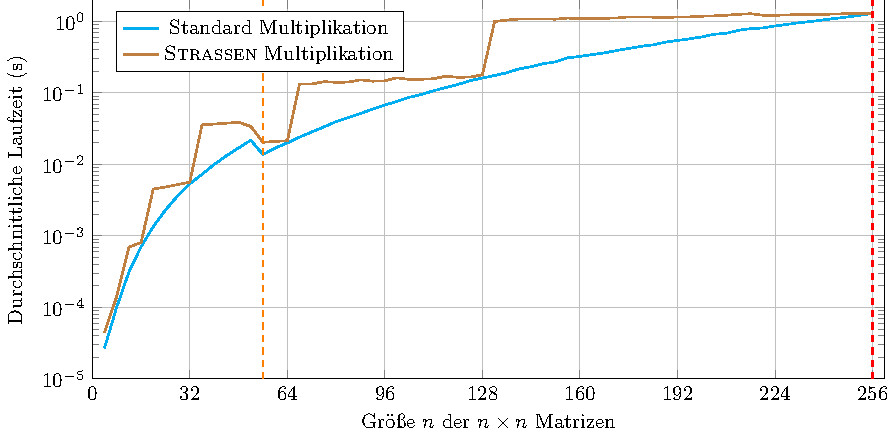
\includegraphics[width=1.0\textwidth]{results.pdf}
	\label{fig:time-comparison}
\end{figure}

Die Abbildung \ref{fig:time-comparison} zeigt die Verläufe der Laufzeit beider Matrixmultiplikationen. Für $n = 56$ liefen sowohl die ursprüngliche als auch \textsc{Strassen}s Multiplikation schneller als für vorherige $n < 56 = 7 \cdot 8$. \textsc{Strassen} verwendet 7 Matrixmultiplikationen, d. h., 14 Untermatrizen. Wie wäre es, wenn 15 Untermatrizen bzw. Strukturen für eine schnellere Matrixmultiplikation als die von \textsc{Strassen} verwendet würden? Die Idee besteht darin, 15 Untermatrizen bzw. Strukturen in den beiden $n \times n$ Matrizen zu finden, um \textsc{Strassen}s Laufzeit zu verbessern. Betrachte dazu die Diagonale der Matrix $B$, um nur 5 statt 7 Matrixmultiplikationen durchzuführen, wodurch eine Laufzeit im Exponenten von $n$ von $2,3219$ statt $2,807$ erreicht wird. Betrachtet man $P_2 = (c + d) \cdot e$ und $P_5 = (a + b) \cdot h$, dann fällt auf, dass $P_2$ durch $P_6$ und $P_1$ ermittelt werden kann und $P_5$ durch $P_1$ und $P_7$. Dazu müssen $P_1$, $P_6$ und $P_7$ berechnet werden bevor $P_2$ und $P_5$ ohne Multiplikation bestimmt werden können. Da nur 5 Matrixmultiplikationen verwendet werden kann das Ergebnis der Laufzeitanalyse wiederverwendet werden mit dem Unterschied, dass 
\begin{align*}
	\vphantom{\rule{0pt}{2.5ex}} T(n) &= 5^{\log_{2}n} \: T\Big(\frac{n}{2^{\log_{2}n}}\Big) + cn^2 \: \sum_{i = 0}^{\log_{2}n-1} \left(\tfrac{5}{4}\right)^i
	\vphantom{\rule{0pt}{2.5ex}} = n^{\log_{2}5} \: T(1) + cn^2 \:\frac{\left(\tfrac{5}{4}\right)^{\log_{2}n} - 1}{\tfrac{5}{4} - 1}
	\vphantom{\rule{0pt}{2.5ex}} = O\left(n^{2.3219}\right).
\end{align*}
Dazu wird der Algorithmus von \textsc{Strassen} zu \textsc{Strassen-25} so geändert, dass $P_6$ und $P_7$ in Zeile 7 und 8 berechnet werden bevor $P_2$ und $P_5$ in Zeile 9 und 10 ermittelt werden.
\begin{algorithm}
	\caption{\textsc{Strassen-25}$(A, B)$}
	\label{alg:strassen}
	\begin{algorithmic}[1]
		\Require $\langle A, B \rangle$, mit $n \times n$ Matrizen $A$, $B$, $n = 2^k$, $k \in \mathbb{N}$
		\Ensure $\langle C, A_{ij}, B_{ij} \rangle$, mit Produktmatrix $C = AB$ und $A_{ij}$, $B_{ij}$
		\If{$n = 1$} $C = AB$ %\Comment{Skalarmultiplikation}
		\State \textbf{return} $C$
		\EndIf
		%\Comment{Matrizen in $n/2 \times n/2$ Blöcke unterteilen}
		\State $A = \begin{pmatrix} A_{11} & A_{12} \\ A_{21} & A_{22} \end{pmatrix}$
		\State $B = \begin{pmatrix} B_{11} & B_{12} \\ B_{21} & B_{22} \end{pmatrix}$
		%\Comment{Berechne die 7 Produkte rekursiv}
		\State $P_1 = \textsc{Strassen-25}(A_{11} + A_{22}, B_{11} + B_{22})$, $P_1 = \langle C^{'}, A^{'}_{11}, A^{'}_{22}, B^{'}_{11}, B^{'}_{22} \rangle$
		\State $P_6 = \textsc{Strassen-25}(A_{21} - A_{11}, B_{11} + B_{12})$, $P_6 = \langle C^{'}, A^{'}_{21}, A^{'}_{11}, B^{'}_{11}, B^{'}_{12} \rangle$
		\State $P_7 = \textsc{Strassen-25}(A_{12} - A_{22}, B_{21} + B_{22})$, $P_7 = \langle C^{'}, A^{'}_{12}, A^{'}_{22}, B^{'}_{21}, B^{'}_{22} \rangle$
		\State $P_2 = A^{'}_{21}A^{'}_{22} + A^{'}_{22}B^{'}_{11}$ von $P_6$, $P_1$ 
		\State $P_5 = A^{'}_{11}B^{'}_{22} + A^{'}_{12}B^{'}_{22}$ von $P_1$, $P_7$
		\State $P_3 = \textsc{Strassen-25}(A_{11}, B_{12} - B_{22})$, $P_3 = \langle C^{'}, A^{'}_{11}, B^{'}_{12}, B^{'}_{22} \rangle$ 
		\State $P_4 = \textsc{Strassen-25}(A_{22}, B_{21} - B_{11})$, $P_4 = \langle C^{'}, A^{'}_{22}, B^{'}_{21}, B^{'}_{11} \rangle$ 
		% \Comment{Berechne die Blöcke von $C$}
		\State $C_{11} = P_1 + P_4 - P_5 + P_7$
		\State $C_{12} = P_3 + P_5$
		\State $C_{21} = P_2 + P_4$
		\State $C_{22} = P_1 - P_2 + P_3 + P_6$
		\State \textbf{return} $C = \begin{pmatrix} C_{11} & C_{12} \\ C_{21} & C_{22} \end{pmatrix}$
	\end{algorithmic}
\end{algorithm}

Bei der Analyse der gemessenen Laufzeit des in Python implementierten Algorithmus \textsc{Strassen-25}$(A, B)$ ist zu erwarten, dass mit 5 Matrixmultiplikationen weniger Laufzeit gemessen wird als mit \textsc{Strassen}$(A, B)$. 
\end{document}